% Discuss the PEAR work and how it is relevant

\chapter{Physically Enhanced Authentication Ring}
\label{chapter:pear}

\section{Overview}
In this section, we present the definition, design, and implementation of the PEAR system. The presentation is this chapter
follows after~\cite{PEAR}.

One problem that is present when using computers is that users typically are not aware of the security of the system
they are using. For instance, an attacker could have installed a key logger on a user's system to harvest every user name
and password they have. Even with the best security systems on the machine in place, if the attacker is able to capture
a user's keystrokes, the other security is moot. 

A way to prevent this type of attack is by using an external device or an alternate channel to enter sensitive information,
such as passwords or credit card numbers. In this way, if a key logger or the original system is compromised, the attacker
will not be able to recover those passwords, credit cards, or other sensitive information.

PEAR, or Physically Enhanced Authentication Ring, was designed to counteract this key logger threat to a system. In addition
to defending against key loggers specifically, it increases security in general because it is the second part of a ``two factor
authentication" system. It also is a physical system, specifically a peripheral physical system, since it incorporates its
own processing and interacts with the user's normal computer system. Thirdly, the PEAR system incorporates a PUF device,
so it is a good example of when PUF technology is useful.

From a high level perspective, a PEAR device is a device consisting of a PUF, a keypad, and some supporting circuitry. When
a user wishes to log on to a given service, rather than using the keyboard for a password, he enters a 4 digit PIN on the PEAR
device. The PEAR device then executes the PUF and then initiates a zero-knowledge proof of knowledge with the service
provider. Note that no sensitive data is actually input to the PC, which potentially has a key logger. Any data that the PC
is requested to ferry between the PEAR device and the service provider is encrypted, so recording this data does not reveal
any information.

The typical use case is that a user requests a PEAR device from a service provider, such as a bank. The bank then configures
and mails the PEAR device to the user. The user sets his PIN number on the device and completes the enrollment protocol.
Then, when he desires to use the service, he requests the authentication protocol. He enters his PIN into the PEAR device
and the device then executes the rest of the authentication protocol. If successful, the service provider then allows
the user to access the service. 
Note that if a user already has a PEAR device from another service provider, he can easily use the same device for another
service; he simply must re-execute the enrollment procedure and enter a new PIN for the new service (or use the old PIN).

The system works by having every service provider associated with an ID number of some kind. Each user of the service will
also have an ID number associated with it. This allows both parties to identify themselves to each other.

\section{Protocol Details}
The PEAR system consists of two parts, an enrollment step, which is executed once initially and then an authentication step,
which is executed every time the user desires to use the service.
Table~\ref{tab:pearprotocol} presents a formalized description of the protocols, while Figure~\ref{fig:pearenrollment}
and Figure~\ref{fig:pearauthentication} give graphical representations of the different stages occurring.

As seen in the diagrams below, the four players in the PEAR system are the user himself, the PEAR device, the user's computer,
and the service provider. Note that the user's computer and the service provider are assumed to be connected over the Internet.

\begin{figure}[!ht]
\centering
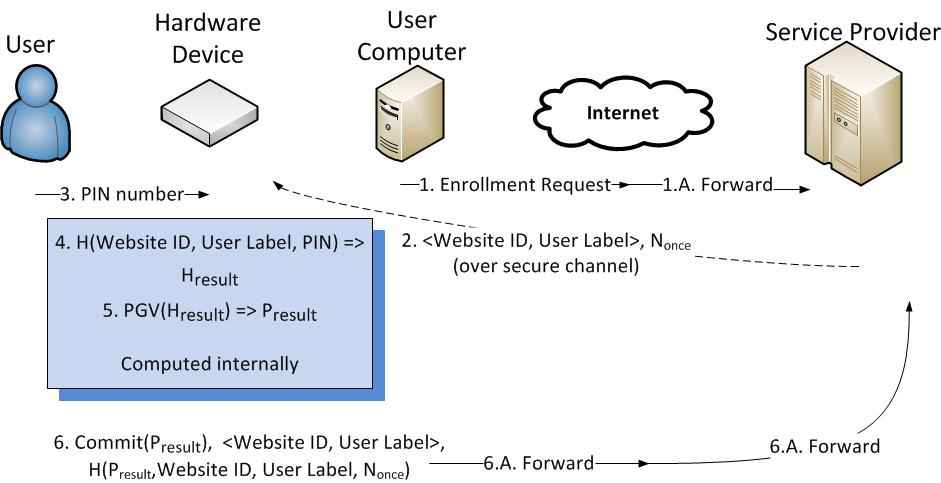
\includegraphics[width=400px]{images/enrollment.jpg}
\caption{The enrollment stage of PEAR}
\label{fig:pearenrollment}
\vspace{-25pt}
\end{figure}
\FloatBarrier

The user initially requests an enrollment procedure from the service provider. The service provider then sends the tuple
of $<Website ID, User Label>$ and a nonce to the PEAR device directly, over a secure channel. The user then enters his
new PIN number to the PEAR device. Once the PEAR device has these different pieces of information, it is able to execute
the steps contained inside the blue box in the diagram. All the pieces of information are hashed together. The resulting
hash is then used as input to the Password Generator and Verifier (PGV). Note that a PUF is an acceptable PGV. The results
from the PGV are then used in a commitment protocol. In addition to sending the results of the commitment to the service
provider, the device also sends the $<Website ID, User Label>$ tuple and a hash of the tuple combined with the committed value.

An interesting point to note is that during the enrollment stage, an ``out of band" communication is required to deliver
the combination of the service provider's ID, the user's corresponding ID for that service, and a nonce value. This could
be done by installing these values on the hardware device before it is given to an end user. For instance, if PEAR was being
used with a bank, the bank might install these values before mailing the device to the user. If the user was adding a new
service to a PEAR device he already had, the tuple of $<Website ID, User Label>$ and the nonce might be delivered through
post or given over the phone to the user. The key point is that they are not delivered over the same channel as will be
used for the rest of the protocols (such as the Internet), since if an attacker is able to recover these values, he would
be able to make a fraudulent account.

\begin{table}[!ht]
\centering
\label{tab:pearprotocol}
\caption{Formalized version of the PEAR protocols}
\noindent\makebox[\textwidth]{%
\begin{tabular}{|l|}
\hline
{\sf Enroll}($U$) --- Device $T$ (using input data from user $U$) computes a \\commitment and enrolls the results with $S$. \\
\hline
$\bullet$ $C$ requests enrollment from $S$ \\
$\bullet$ $S$ sends the tuple $<$Label, ID$>$ and nonce $N$ to $T$ over a secure channel \\
$\bullet$ $U$ sends PIN to $T$ \\
$\bullet$ $T$ computes {\sf H}(ID, Label, PIN) as $H_{result}$ \\
$\bullet$ $T$ executes {\sf PGV}($H_{result}$) as $P_{result}$ \\
$\bullet$ $T$ sends {\sf Commit}($P_{result}$), $<$Label, ID$>$, {\sf H}({\sf Commit}($P_{result}$),Label,ID,$N$) to $S$, \\via $C$ \\
\hline
\hline
{\sf Authenticate}($U$) --- Device $T$ (using input data from user $U$) \\authenticates itself as a registered user of $S$. \\
\hline
$\bullet$ $C$ initiates the authentication request from $S$ \\
$\bullet$ $S$ sends the tuple $<$Label, ID$>$ and {\sf Chal}($P_{result}$) to $T$ \\
$\bullet$ $U$ sends PIN to $T$ \\
$\bullet$ $T$ computes {\sf H}(ID, Label, PIN) as $H_{result}$ \\
$\bullet$ $T$ executes {\sf PGV}($H_{result}$) as $P_{result}$ \\
$\bullet$ $T$ responds with {\sf Prove}($P_{result}$), which $C$ forwards to $S$ \\
\hline
\end{tabular}
}
\end{table}
\FloatBarrier

\begin{figure}[!ht]
\centering
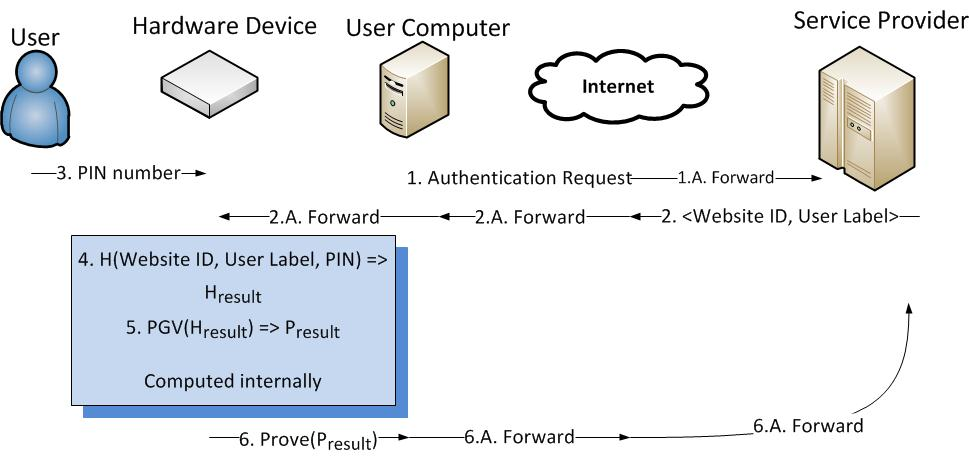
\includegraphics[width=400px]{images/auth.jpg}
\caption{The authentication stage of PEAR}
\label{fig:pearauthentication}
\vspace{-25pt}
\end{figure}
\FloatBarrier

\section{Additional Usage Scenarios}
In addition to allowing authentication over an insecure channel as originally intended, PEAR also provides two other
beneficial usage scenarios.

\subsection{Unlinkability Property}
Currently, users may be enrolled under several service providers for various reasons. Each service provider might
hold some pieces of sensitive information about the user, but not necessarily every piece of sensitive information.
However, if the two service providers were to collude, they would be able to learn a lot more about an individual
user, which is not desirable.

\begin{figure}[!ht]
\centering
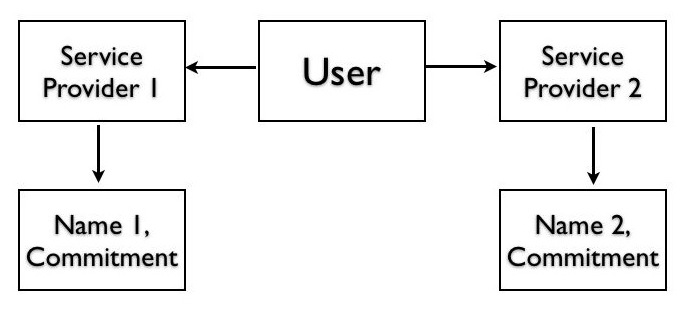
\includegraphics[width=400px]{images/pearpics.jpg}
\caption{The unlinkability property of PEAR}
\label{fig:pearunlinkability}
\vspace{-25pt}
\end{figure}
\FloatBarrier

As such, it is desirable to only give information out in a way such that service providers cannot collude to violate
a user's privacy. The PEAR system provides this capability. When enrolling with two different service providers,
the user would use a different screen name with each and send a commitment. Because the commitments do not
leak any information (and the website IDs and user IDs are different), even if the service providers colluded, they would
not be able to determine which pair of accounts belong to the same user very easily.

\subsection{Organizational Anonymity}
Another issue that frequently arises is that users may need to contact a party outside of their organization, but
they do not want to be individually identified; they wanted to be recognized as a university member only. For instance,
a Purdue student may wish to access the ACM digital library. She does not want to register with the library as an
individual; she simply wants access granted due to her Purdue affiliation.
However, the university, or whoever the authority is, still needs to maintain some sort of auditing capability.

PEAR is able to fulfill this use case as well. Users will use a PEAR device to enroll under the authority (the university
in the previous example). When they desire some service (such as digital library access), users will use PEAR to 
authenticate to the authority, who will then authenticate to the service provider on their behalf.

\begin{figure}[!ht]
\centering
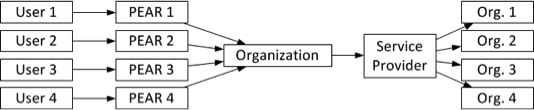
\includegraphics[width=400px]{images/pearorgnaizational.jpg}
\caption{The organizational anonymity aspect of PEAR}
\label{fig:pearorganizational}
\vspace{-20pt}
\end{figure}
\FloatBarrier

In this way, users remain anonymous to the outside world and external service providers. However, if a problem occurs,
the authority can still hold users accountable for any actions they took.

\section{Security Considerations}
Several lemmas are presented below which address various different security aspects of the PEAR system.
Following the lemmas is a discussion of some of the different security issues facing physical systems that
were discussed in Chapter~\ref{chapter:physicalsystems} and how the lemmas relate to those concerns.

\subsection{Lemmas}
\noindent \textbf{Lemma 1.} \\
\noindent \emph{A man-in-the-middle attacker cannot recover any useful data communicated over the network between the
service provider and the computer.} \\
{\bf Proof:}  The only data that is transmitted between the computer and network is the tuple containing the service
ID and the user's ID initially and then steps of the zero-knowledge proof (see Figures~\ref{fig:pearenrollment} and
\ref{fig:pearauthentication}). The tuple will only be sent during authentication, so we can assume that users are already enrolled.
An attacker gains nothing by intercepting the tuple during authentication, since it still requires both the user PIN
number and the device itself to impersonate a user. Intercepting the steps of the zero-knowledge proof also gives him
no information since these zero-knowledge protocols do not reveal any information about the committed value.
%\hfill$\square$ \\

\noindent \textbf{Lemma 2.} \\
\noindent \emph{A man-in-the-middle attacker cannot recover any useful data communicated between the user computer and
the device.} \\
{\bf Proof:}  As shown in Figures~\ref{fig:pearenrollment} and \ref{fig:pearauthentication}, the only data that is being transmitted over this channel is
the tuple from the server and the zero-knowledge steps. As shown in Lemma 1, an attacker cannot gain any useful
information from this. 
Also note that the PUF secret is never transferred outside of the device, but rather a commitment or
proof is sent. As such, a MITM attack would not reveal the user's secret, but only the various steps of
the zero-knowledge proofs, which are secure against MITM attacks. In addition, the service provider does not even ever
know the user's PIN.%\hfill$\square$ \\

\noindent \textbf{Lemma 3.} \\
\noindent \emph{An active man-in-the-middle attacker cannot recover any useful information by modifying data between
the device and computer or computer and network during the authentication stage.} \\
{\bf Proof:}  An attacker who modifies the tuple being sent to the device or computer from the network would cause the
device to create an incorrect zero-knowledge proof. This would disrupt the user's ability to authenticate. However,
the attacker would not be able to glean any information from the proof generated from this modified tuple, due to the
use of the zero-knowledge proof.
Note that an attacker would be able to recover useful information if it could modify the tuple during enrollment. It
could substitute a malicious tuple for the valid tuple, which would cause users to be authenticating to the MITM, rather
than the service provider. We avoid this problem by requiring that the tuple be sent securely during enrollment.
%\hfill$\square$ \\

\noindent \textbf{Lemma 4.} \\
\noindent \emph{A PPT adversary can impersonate a legitimate user to the server with only negligible probability.} \\
{\bf Proof:}   As the final authentication step is to complete a zero-knowledge proof, an attacker would have to be able
to defeat a zero-knowledge proof, which happens only with a negligible probability if an attacker does not know the
user's secret.%\hfill$\square$ \\

\noindent \textbf{Lemma 5.} \\
\noindent \emph{Given physical access to the device, an attacker could impersonate the legitimate user with only
negligible probability.} \\
{\bf Proof:}  If an attacker had access to the device, it would not be able to compute the proper hash value unless it
supplied the correct PIN to the device. If the attacker attempted a brute force attack on the user's PIN,
it would be trivial for a server to detect and disable the user's account temporarily. As long as the key space for the
PIN is sufficient, this attack is not realistic.%\hfill$\square$ \\

\noindent \textbf{Lemma 6.} \\
\noindent \emph{A legitimate user can authenticate to a legitimate $S$, except with negligible probability.} \\
{\bf Proof:}  As a legitimate user would have access to the user PIN and a valid tuple from the server, he would be
able to successfully complete the zero-knowledge proof, thus authenticating.%\hfill$\square$ \\

\noindent \textbf{Lemma 7.} \\
\noindent \emph{An attacker cannot enroll using an existing or past user's credentials, except with negligible
probability.} \\
{\bf Proof:} An attacker would be able to capture a user's tuple during authentication. It is plausible that he could
attempt to enroll using this tuple. To prevent this, when the service provider issues the tuple initially, it also
provides a nonce. During the enrollment protocol, the user submits the committed value, the tuple, and a hash of the
tuple, nonce, and committed value. The service provider will verify that this tuple is valid. If the tuple is not
valid or has already been enrolled, the service provider denies the enrollment request.%\hfill$\square$ \\

\subsection{Man in the Middle}
One of the considerations for system design is the presence of a man in the middle (MITM) attacker. If the MITM
attacker is able to capture sufficient sensitive data, he could potentially compromise the security and integrity
of the system. 

Lemmas 1, 2, and 3 address the capabilities of an MITM attacker. Notably, since the attacker would only capture
public information or interim steps of the zero knowledge proof, he is unable to recover anything of interest.
However, an active MITM attacker would be able to drop all traffic between the various parties and commit a
denial of service attack, though this case is not of great interest.

\subsection{Replay Attacks}
It is important to ensure that an attacker cannot record communication and then replay these communications
later on.

Lemma 7 addresses this type of threat. Since the enrollment stage requires a nonce, it is not possible
to record a user's tuple from the authentication step and use that to enroll. Lemma 1, 2, and 3 make mention
of the fact that only interim steps of the zero knowledge proof would be recoverable, which are not usable
in a replay attack.

\subsection{Impersonation}
Impersonation is another threat that must be considered; it is unacceptable if an adversary is able to pose as
the service provider or as a user.

Lemmas 4 and 5 discuss the threat of impersonation. Simple brute force impersonation of a user to a service
provider would require defeating a zero knowledge proof, which is computationally unfeasible. If the attacker
was able to steal the physical device, he would be able to execute the zero knowledge proof, assuming he could
guess the user's PIN. If a brute force attack was used, the service provider would easily be able to detect it.

\section{Implementation}
From a high level view, Figure~\ref{fig:peararchitecture} describes the initial implementation of a PEAR enabled device.
The Saxo-L board from KNJN.com~\cite{KNJN} was used to do this work. The board contained both an FPGA and an ARM
micro controller. The FPGA was used to implement the PUF device and supporting circuitry. The ARM micro controller
was used to do the general purpose computation, including all the different cryptographic processing. The two
were connected to each other with a Serial Peripheral Interface. A keypad for entering PINs was connected using a
breadboard and directly wiring it to I/O pins of the ARM. The entire system was then connected to the PC over
a USB connection.

\begin{figure}[!ht]
\centering
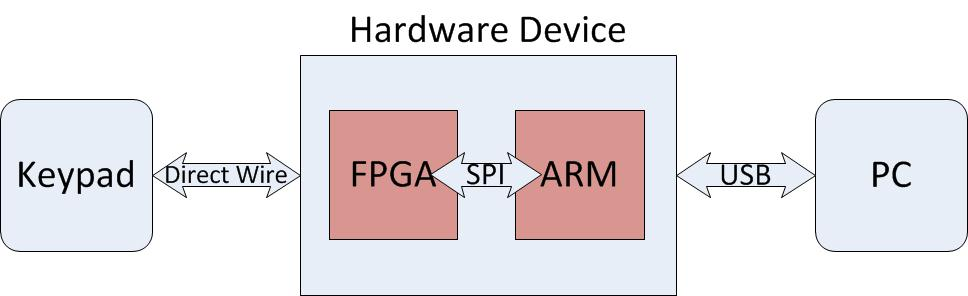
\includegraphics[width=400px]{images/pearimpl.jpg}
\caption{Implementation of a PEAR device}
\label{fig:peararchitecture}
\vspace{-20pt}
\end{figure}
\FloatBarrier

The entire Saxo-L board is 44mmx60mm, which is smaller than a typical credit. As such, a production level PEAR
device could be implemented in a variety of user friendly sizes. A dongle or a smart card are two possible form
factors that would be usable and convenient. The keypad for PINs could be overlayed as an array of touch-capacitive 
buttons on top of either form factor as well.

\subsection{Limitations}
Because the initial implementation was proof of concept, there are several ways it could be improved. Several
vulnerabilities are also present that were discussed in Chapter~\ref{chapter:physicalsystems}.

One glaring shortcoming is the fact that the PUF and the ARM are connected over an SPI interface which is completely
open on the Saxo-L board. As such, an adversary could easily put logic probes on the SPI bus and record the PUF
challenge/response values as they were transmitted to the ARM, since they are sent unencrypted. There are a few
ways to remedy this. 

One solution is to put sorts of tamper proofing in place, such as potting, power filtering, among others. 
This would be effective, but would most likely be expensive and not completely effective. Another solution would
be to encrypt the traffic being sent over the SPI bus. This would be fairly easy to do, but would impose some
computational overhead on the entire device, which may or may not be acceptable. 

The ideal solution to this problem is to incorporate the micro controller onto the same chip as the PUF itself. This
is possible since there are ``soft core" versions of ARM available which can be instantiated on the FPGA. Additionally,
Altera (who makes the FPGA on the Saxo-L) provides a soft core micro controller for their FPGAs, as do many other
FPGA vendors. This is probably the best solution since it eliminates the need for two discrete chips, since both portions
can be put in one FPGA. It is still possible to use the same SPI bus concept, but the SPI bus will be internal to the
FPGA, so it will not be possible to put logic probes on it. If an attempt is made to strip portions of the FPGA to
insert probes, this will likely disturb the PUF and corrupt it, so any results will be unhelpful. Tampering with the FPGA
and its relation to the PUF inside was discussed in Chapter~\ref{chapter:pufoverview} in more detail.

If the entire device was incorporated on to an FPGA, there would need to also be some sort of power filtering done.
This would prevent differential power analysis attacks from being done on the cryptographic portions of the FPGA.

While it is necessary to prevent tampering to some degree, Lemma 5 means that a large amount of tamper proofing
is not necessarily needed. The device is in its most vulnerable state after the PIN has been entered and the device is
executing the zero knowledge proof. If an attacker has attached logic probes and other tools necessary to conduct
many kinds of attacks, it would be very obvious to the legitimate users, who would then refuse to enter their PINs.

\section{Future Work}
The PEAR system as it exists is quite functional. However, some extensions could be done as future work to improve
the system. 

One such improvement is the concept of ``transaction levels". Typically, service providers grant a user all services after
he has logged in, regardless of the sensitivity of the requested action. For instance, a web application will require a
user to log in before starting a new session, after which, all requests are granted. Transaction levels are the use of
different credentials or the requiring of re-authentication upon requests for certain actions. 

In a banking website 
example, one transaction level may allow a user to perform non-destructive operations, such as checking an account
balance. However, for destructive operations, such as making an online bill payment, a different transaction level
would be needed.

Transaction levels would be possible to implement so that a user only needed one physical PEAR device. This is
desirable, because requiring a user to carry around multiple PEAR devices is not necessarily realistic.

Properly implementing transaction levels would require addressing a number of technical challenges. First, we would 
need an appropriate policy language to capture the behavior. Next, we would need to explore how to present the user 
with a usable interface that abstracts the behavior. Finally, we would need to consider the trade-offs in 
usability and security that would result from applying these approaches.